\documentclass[10pt,twocolumn,letterpaper]{article}

\usepackage{cvpr}
\usepackage{times}
\usepackage{epsfig}
\usepackage{graphicx}
\usepackage{subcaption}
\usepackage{amsmath}
\usepackage{amssymb}
\usepackage{dsfont}
\usepackage{bm}
\usepackage{bbm}
\usepackage{amsfonts,amscd}
\usepackage{amssymb,amsmath,amsthm,enumerate}
\usepackage{physics}

\usepackage{tikz}
\usetikzlibrary{calc}
\usetikzlibrary{shapes,arrows}

\DeclareMathOperator*{\argmax}{arg\,max}
\DeclareMathOperator*{\argmin}{arg\,min}

% Include other packages here, before hyperref.

% If you comment hyperref and then uncomment it, you should delete
% egpaper.aux before re-running latex.  (Or just hit 'q' on the first latex
% run, let it finish, and you should be clear).
\usepackage[breaklinks=true,bookmarks=false]{hyperref}

\cvprfinalcopy % *** Uncomment this line for the final submission

\def\cvprPaperID{****} % *** Enter the CVPR Paper ID here
\def\httilde{\mbox{\tt\raisebox{-.5ex}{\symbol{126}}}}

% Pages are numbered in submission mode, and unnumbered in camera-ready
%\ifcvprfinal\pagestyle{empty}\fi
\setcounter{page}{1}
\begin{document}

%%%%%%%%% TITLE
\title{Deep Reinforcement Learning for Bearing-only Radiolocation}

\author{Cedrick Argueta \\
{\tt\small cdrckrgt@stanford.edu}
% For a paper whose authors are all at the same institution,
% omit the following lines up until the closing ``}''.
% Additional authors and addresses can be added with ``\and'',
% just like the second author.
% To save space, use either the email address or home page, not both
}

\maketitle
%\thispagestyle{empty}

%%%%%%%%% ABSTRACT
\begin{abstract}
Unauthorized drones present a danger to airports and disaster areas.
Localization and tracking of these unauthorized drones reduces some of this danger.
It is possible to use a drone outfitted with with commericial antennas and radios to autonomously localize other drones.
In this work, we show preliminary results detailing how a drone with this equipment may use deep reinforcement learning to perform path planning in a localization task.
\end{abstract}

\section{Motivation}
Tracking a moving radio target, such as a drone, is a useful and non-trivial task.
An unauthorized drone could be disrupting airport operations, causing delays or interfering with aircraft.
This task is not limited to tracking other drones: a wildlife radio tag could help with studying migration patterns of migrant animals.
In this work, we model this problem as a dynamic system and apply a continuous control reinforcement learning algorithm, deep deterministic policy gradient (DDPG), as a solution method.

This work is intended to be a variant to work that I am pursuing for my honors thesis.
My honors thesis revolves around this problem in the discrete setting, where there is imperfect information received from the environment.
My honors thesis also involves the use of a sensor that gives very little information on the environment, resulting in a difficult sensor integration problem.

Here I intend on using a sensor that provides much more information of the environment, resulting in an easier version of my honors thesis.
This balances the difficulty of considering continuous control over discretized control.


\section{Mathematical Models}
\label{sec:models}
This section described the mathematical models used to formalize the system.

\subsection{Drone Dynamics}
The drone dynamics are exactly those described in \cite{dronehunter}.
The seeker drone state at time $t$ is $x_t = [x_t^n, x_t^e, x_t^h]^\intercal$, where $x_t^n$ and $x_t^e$ are the seeker's north and east coordinates and $x_t^h$ is the seeker's heading measured east of north.
The state described here does not contain velocity or altitude as simplifying assumptions.
The drone follows a first-order motion model, so the state after applying a control input $u_t$ for duration $\Delta t$ the new state is
\begin{equation}
x_{t + \Delta t} = x_t + u_t\Delta t
\end{equation}

The target drone state at time $t$ is $\theta_t = [\theta_t^n, \theta_t^e]^\intercal$, where $\theta_t^n$ and $\theta_t^e$ are the target's north and east coordinates.
The target drone is assumed to move with a constant velocity $\dot{\theta} = [\dot{\theta_t^n}, \dot{\theta_t^e}]^\intercal$.
The drone follows a first-order motion model, so the state after $\Delta t$ is
\begin{equation}
\theta_{t + \Delta t} = \theta_t + \dot{\theta_t}\Delta t
\label{target_dynamics}
\end{equation}

\subsection{Sensor Model}
The bearing from the seeker drone to the target drone is 
\begin{equation}
\beta_t = \arctan{\frac{\theta_t^e - x_t^e}{\theta_t^n - x_t^n}}
\end{equation}
when measured east of north.
Configured properly, the directional antenna and omnidirectional antenna can give estimates of the relative bearing of the target drone.

At time $t$, the seeker drone makes measurement $z_t \sim \mathcal{N}(\beta_t - x_t^h, \sigma^2)$, which is a bearing in the interval $[0^{\circ}, 360^{\circ}]$.
It is assumed that these measurements are normally distributed about the true relative bearing with some variance to account for sensor error.

My honors thesis work uses a sensor that only provides a (noisy) boolean representing whether the target is in front of or behind the seeker, which provides much less information than a relative bearing measurement.
The sensor model used here was verified experimentally in \cite{sensor_modality}.

\subsection{Particle Filter}
The seeker drone maintains a belief of the possible location of the target drone, which is modeled with a particle filter.
Belief at time $t$ is represented by a set of $N$ particles, each representing a hypothesis of the target drone's pose.
Updates are made to the particle filter at every timestep to improve the belief's accuracy.

The belief update consists of three steps. 
The first step is the prediction step, where each particle is propagated according to the dynamics described in equation \ref{target_dynamics}.
Noise is added to the dynamics to prevent particle deprivation, a situation that arises when all particles converge to a hypothesis that doesn't accurately represent the true state.
The second step is the weighting step, where each particle is assigned a weight according to how probable an observation $z_t$ is given the particle's position.
The third step is resampling, where particles are sampled according to these weights with replacement.
In this work, we use stratified resampling to aid in maintaining an accurate estimate of the target while ensuring resiliency to particle deprivation.

\subsection{Belief Markov Decision Process}

The planning algorithm uses the partially observable Markov decision process (POMDP) framework for analysis.

A POMDP comprises a state space $\mathcal{S}$, an action space $\mathcal{A}$, a reward function $R$, and a transition function $T$ defining the transition between states.
An agent is unable to observe the true state $s_t$ directly and instead makes an observation $\omega \in \Omega$ conditioned on the true state.

Solving a POMDP consists of finding a policy $\pi^*$ such that
\begin{equation}
\pi^* = \argmax_{\pi}{\mathbb{E}\left [ \sum_{t=0}^{\infty}\gamma^{t}R(s_t, \pi(\omega_t)) \right ]}
\label{optimal_policy}
\end{equation}
where $\gamma$ is a discount factor.

POMDPs have a significant disadvantage when formalizing localization tasks.
Rewards that depend on belief of the true state of the system are often difficult to represent in the POMDP framework \cite{dronehunter}.
For this reason, we instead convert the POMDP to a belief-Markov decision process, or belief-MDP.

Belief-MDPs are similar to MDPs where the system state is instead a \textit{belief} of the true system state.
We hereafter model the problem as an MDP where each state is a tuple of the fully observable part of the true state and the belief of the partially observable part of the true state.

\subsection{Formulation}

\subsubsection{States}
Each state is a tuple $s_t = (b_t, x_t)$ where $b_t$ is the seeker's belief and $x_t$ is the seeker's pose.
The seeker's belief is the particle filter mentioned in the previous section.

\subsubsection{Actions}
The seeker is allowed to travel with a constant velocity towards any bearing.
The seeker is also allowed to take no action.

The baseline controllers are discrete methods, and thus can only travel towards some bearings.
Current experiments are run over 24 directions with a null action, resulting in 25 total discrete actions.

\subsubsection{Reward Function}
Our reward function for radiolocation captures the desire to maintain an accurate and precise estimate of the target's location \textit{while also} maintaining an acceptable distance from the target.

A precise belief is one that has low uncertainty over the target's position.
Minimization of this uncertainty is equivalent to minimization of the entropy of the belief distribution.
Particles in the filter are first discretized into $M$ bins.
Entropy can then be defined as:
\begin{equation}
H(b_t) = -\sum_{i = 1}^M\tilde{b}_t[i]\log\tilde{b}_t[i]
\label{entropy_unnormalized}
\end{equation}
where $\tilde{b}_t$ is the proportion of particles in each bin.
We normalize this entropy to be between $0$ and $1$, arriving at
\begin{equation}
H_{n}(b_t) = 1 - \frac{H(b_t)}{\log{M}}
\label{entropy_normalized}
\end{equation}.

An accurate belief is one that has a low tracking error with respect to the true target's state.
Tracking error is
\begin{equation}
E(b_t, \theta_t) = \Vert \mathbb{E}{[ b_t ]} - \theta_t \Vert
\label{tracking_unnormalized}
\end{equation}
but we again normalize the error to be between $0$ and $1$.
We choose to divide by the maximum error in the search domain, which for a domain of length $l$ is $l\sqrt{2}$.
Our normalized tracking error is then
\begin{equation}
E_{n}(b_t, \theta_t) = 1 - \frac{E(b_t)}{l\sqrt{2}}
\label{tracking_normalized}
\end{equation}.

Near-collisions are penalized to encourage the seeker to keep a safe distance.
The penalty term contains only the belief of the belief of the target's position rather than the true target position.
This is to encourage the seeker to maintain a distance from the particles during evaluation.
If the belief is representative of the true state, then the seeker will maintain a safe distance.
If the belief is not representative of the true state, then the seeker will at least maintain a distance from the belief, which still might contain a noisy or partially accurate model of the target's motion.
Our near-collision penalty is
\begin{equation}
C(b_t, x_t) = 1 - \mathop{{}\mathbb{E}}_{b_t} \mathds{1} (\Vert x_t - \theta_t\Vert < d)
\label{collision_penalty}
\end{equation}
where $\mathds{1}$ is an indicator function and $d$ is the safe distance we wish the seeker to maintain.

The terms are combined to produce our full reward function:
\begin{equation}
R(b_t, x_t, \theta_t) = \lambda_1 H_{n}(b_t) + \lambda_2 E_{n}(b_t, \theta_t) + \lambda_3 C(b_t, x_t)
\label{reward_function}
\end{equation}
where $\lambda_1$, $\lambda_2,$ and $\lambda_3$ are coefficients controlling the importance of each term.

\section{Preliminary Experiments}

\subsection{Baseline}
There are two current baselines for this experiment, both discrete.
The first is a greedy method, which iterates over all possible actions and chooses that which maximizes the reward function for that step.
The second is the standard deep Q-networks (DQN) algorithm, which makes Q-learning tractable with continuous observation spaces through the use of neural networks.

The greedy method represents a simple first step towards a solution, while DQN represents a first foray into deep reinforcement learning as a solution space.
Both rely on a discretized action space, which is often done with continuous control problems to make them tractable.

\subsubsection{Greedy Method}
The greedy method performs as expected.
An example run is shown in figure \ref{fig:greedy}.
The greedy method has acculmated rewards from $8.0$ to up to $45.0$.
The seeker will trail the target, concentrating belief behind the target with high tracking error.
This is because the greedy method chooses the best action for that step, without taking into account that the target is moving with some unknown velocity.

The baseline is, however, still useful to illustrate the difficulty of this problem for learning-based systems -- the controller must take into account that the target is moving, and figure out the target's approximate velocity by taking good actions that give the particle filter enough information.

\begin{figure}[h!]
  \centering
  \begin{subfigure}[b]{0.48\linewidth}
    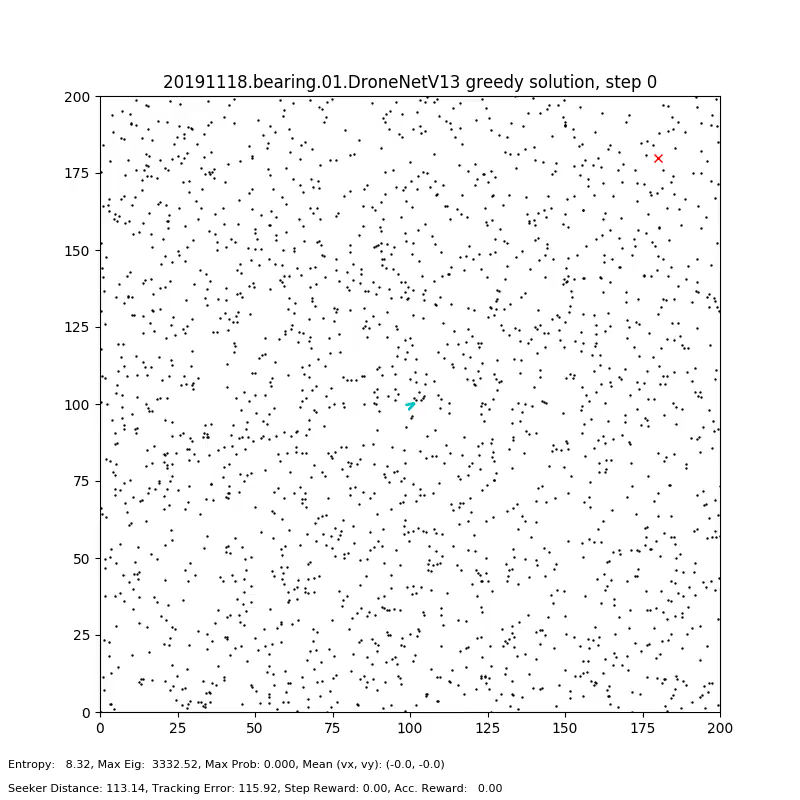
\includegraphics[width=\linewidth]{images/first.png}
    \caption{Initialization.}
  \end{subfigure}
  \begin{subfigure}[b]{0.48\linewidth}
    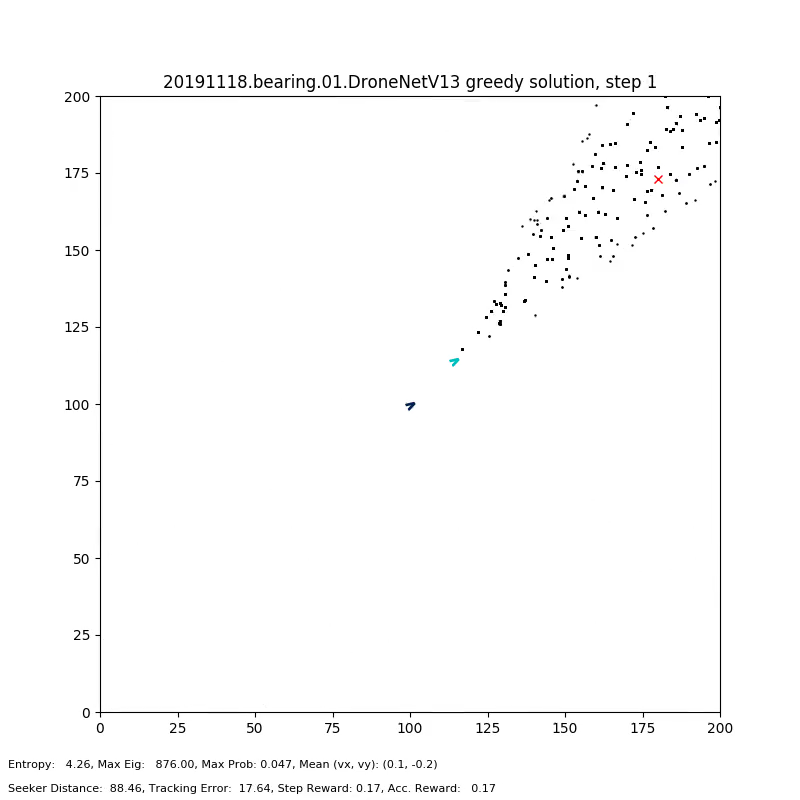
\includegraphics[width=\linewidth]{images/second.png}
    \caption{After some steps.}
  \end{subfigure}
  \begin{subfigure}[b]{0.48\linewidth}
    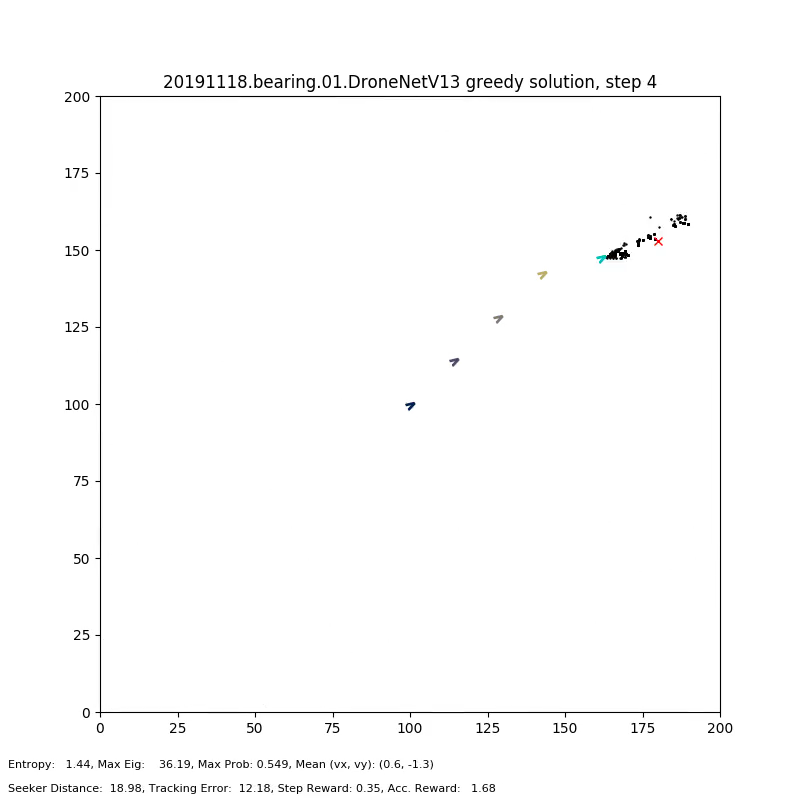
\includegraphics[width=\linewidth]{images/third.png}
    \caption{Belief mostly concentrated.}
  \end{subfigure}
  \begin{subfigure}[b]{0.48\linewidth}
    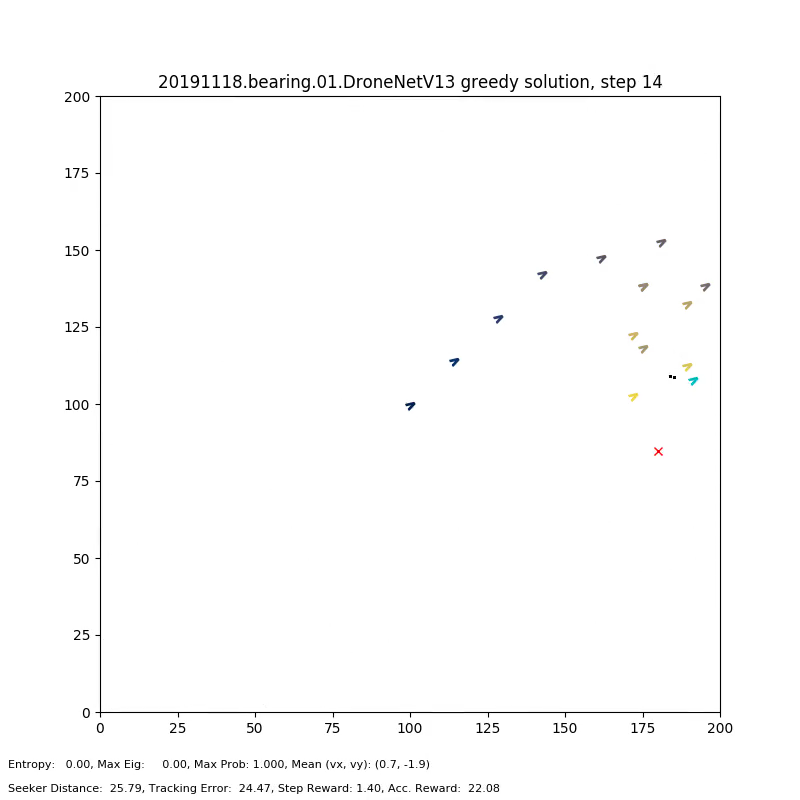
\includegraphics[width=\linewidth]{images/fourth.png}
    \caption{Belief concentrated.}
  \end{subfigure}
  \caption{Progression of states for the greedy solver.}
  \label{fig:greedy}
\end{figure}

\begin{figure}[h!]
  \centering
  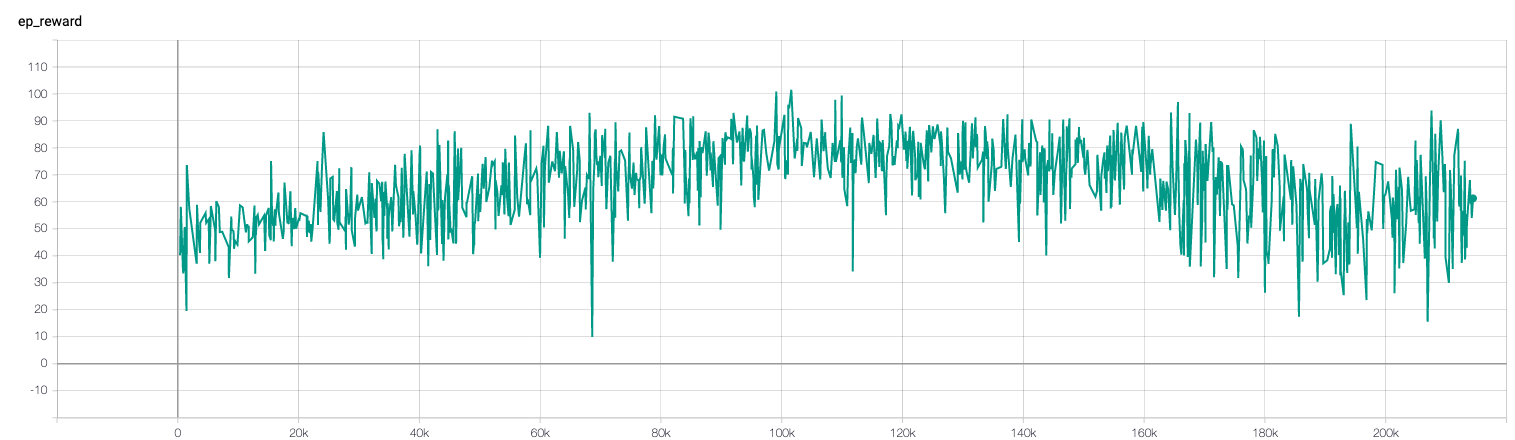
\includegraphics[width=\linewidth]{images/avg_dqn.png}
  \caption{Reward curve over time.}
  \label{fig:avg_dqn}
\end{figure}
\subsubsection{DQN}
An exploration of DQN in this problem reveals that learning-based systems perform relatively better.
It is well known that reinforcement learning models will exploit flaws in reward functions to get the maximum reward \cite{rlblogpost}.
This is especially prevalent in the DQN baseline, where the seeker learns to minimize the entropy of the belief regardless of how good or bad the belief's accuracy is.
Figure \ref{fig:dqn} shows how a higher reward is reached not necessarily by having better subjective performance but by maximizing the entropy reward from our cost function.
Figure \ref{fig:avg_dqn} shows the reward over all training episodes, representing a much higher reward than the greedy method.

The experiments run so far with DQN showcase how important it is to formulate the reward function in a way that incentivizes all the desired behavior without allowing for degenerate cases like this.
While the DQN algorithm shows that a higher total reward is easily attainable by a reinforcement learning algorithm, it also reveals that the reward function must be reworked to incetivize the reduction of tracking error more.
Further testing will need to be done with these baselines to determine a proper reward function that the continuous solution method can optimize well.

\begin{figure}[h!]
  \centering
  \begin{subfigure}[b]{0.48\linewidth}
    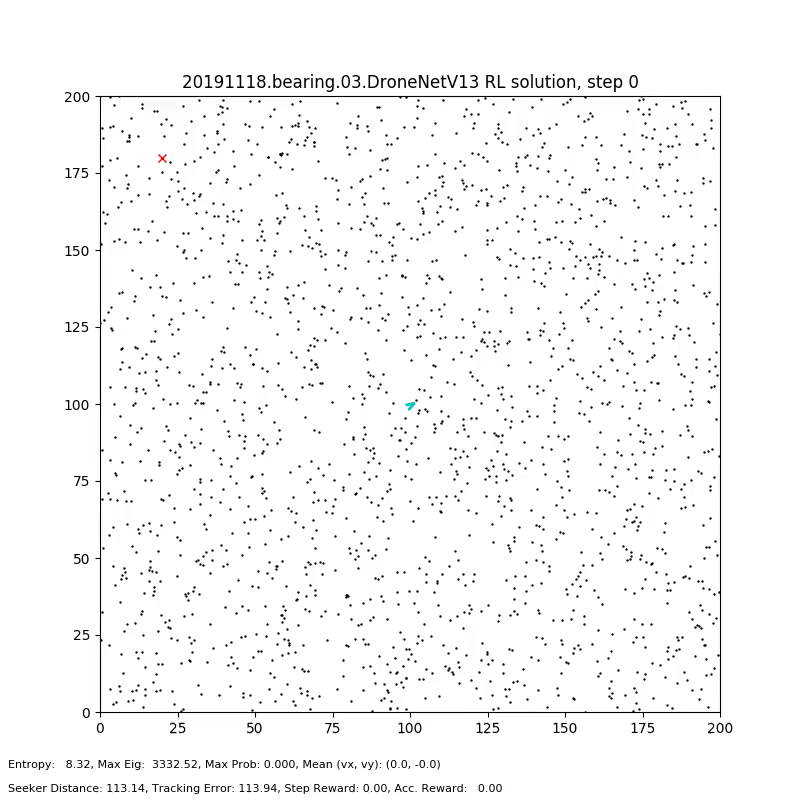
\includegraphics[width=\linewidth]{images/fifth.png}
    \caption{Initialization.}
  \end{subfigure}
  \begin{subfigure}[b]{0.48\linewidth}
    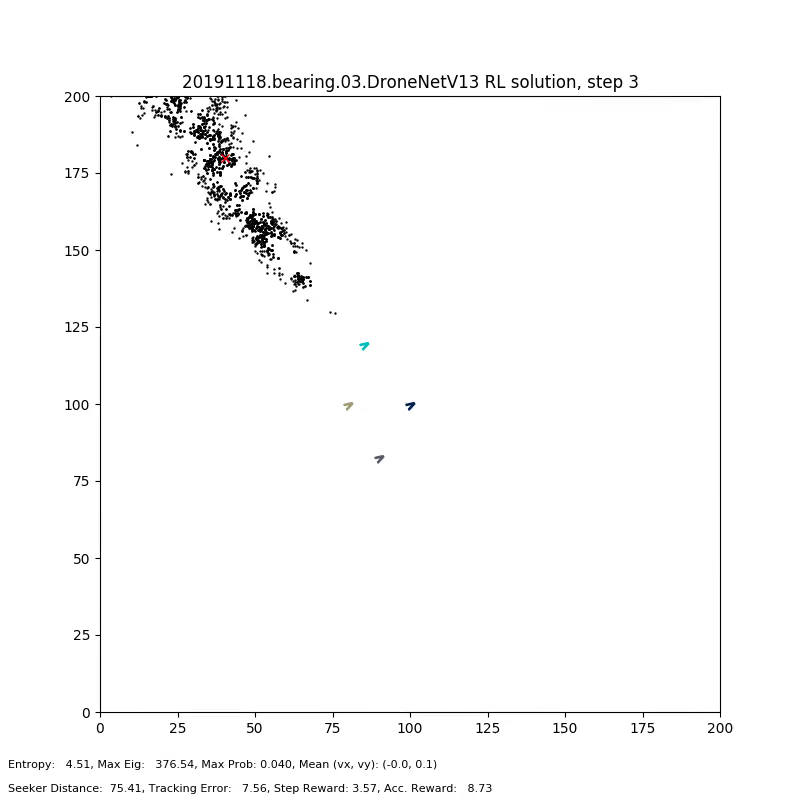
\includegraphics[width=\linewidth]{images/sixth.png}
    \caption{After some steps.}
  \end{subfigure}
  \begin{subfigure}[b]{0.48\linewidth}
    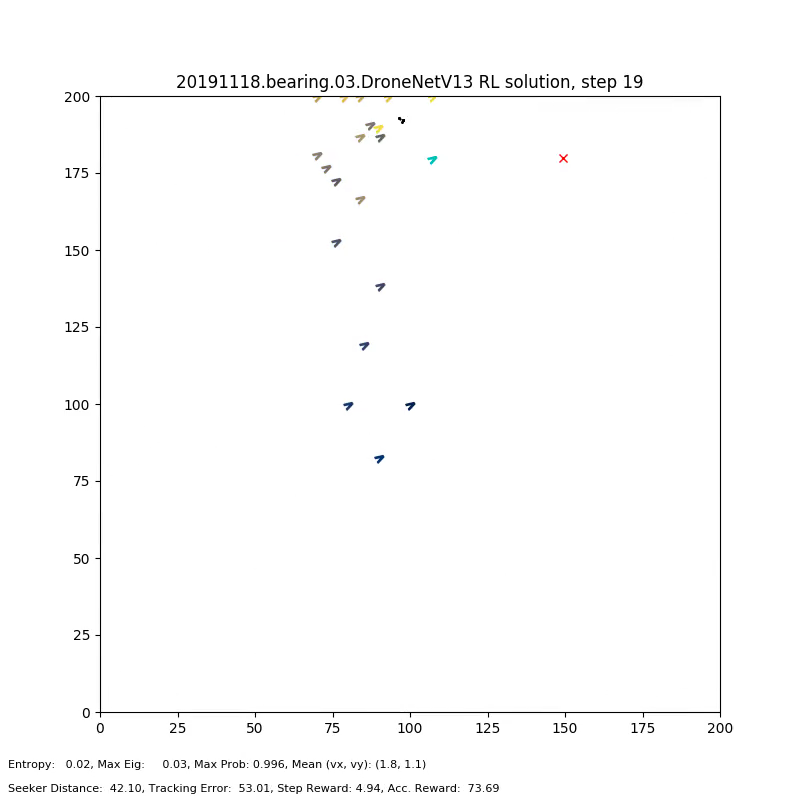
\includegraphics[width=\linewidth]{images/seventh.png}
    \caption{Belief concentrated.}
  \end{subfigure}
  \caption{Progression of states for the DQN solver.}
  \label{fig:dqn}
\end{figure}



\subsection{Secondary Metrics}
Each solution method can be evaluated using the average accumulated reward over all episodes.
However, a number of other metrics can be taken into account as well.
Average time to reach a minimum level of performance (i.e. time to reach 50\% confidence in our belief estimate) can be important when trying to take only approximately optimal steps.
Also of interest is the execution times for different methods: a continuous control algorithm that takes twice as long to produce a control input than a discrete control algorithm might not be worth the tradeoff for finer grained control.
While I don't have these metrics baked into my simulator, I am considering them for the final report.

\subsection{Solution Method}
To solve this problem in the continuous setting, we use DDPG \cite{ddpg} and TD3 \cite{td3} and DQN \cite{dqn}.
This algorithm uses a neural network to approximate the value function and a neural network to approximate the policy.

\subsubsection{Progress so far}
I have written my own implementation of DDPG in PyTorch that is compatible with my simulator, but haven't yet tested it on the full problem.
So far I have only solved the Pendulum environment from OpenAI Gym \cite{gym}.
However, since I've written it in such a way that it interfaces well with my simulator, I will be able to run experiments in the continuous setting soon.

\section{Contributions}
I worked on this project alone.

Again, this project is derivative of my work for my honors thesis, but still represents different challenges. 
The sensor model used is different, specifically this project uses an `easier' sensor model to work with.
Also, my honors thesis so far has only considered discrete control, while the end goal of this project is to do continuous control.
It will be useful to have a functioning implementation of DDPG that I can use in the future for this task.

%%%%%%%%% BODY TEXT
% \section{Introduction}
% 
% Please follow the steps outlined below when submitting your manuscript to
% the IEEE Computer Society Press.  This style guide now has several
% important modifications (for example, you are no longer warned against the
% use of sticky tape to attach your artwork to the paper), so all authors
% should read this new version.
% 
% %-------------------------------------------------------------------------
% \subsection{Language}
% 
% All manuscripts must be in English.
% 
% \subsection{Dual submission}
% 
% Please refer to the author guidelines on the CVPR 2019 web page for a
% discussion of the policy on dual submissions.
% 
% \subsection{Paper length}
% Papers, excluding the references section,
% must be no longer than eight pages in length. The references section
% will not be included in the page count, and there is no limit on the
% length of the references section. For example, a paper of eight pages
% with two pages of references would have a total length of 10 pages.
% {\bf There will be no extra page charges for CVPR 2019.}
% 
% Overlength papers will simply not be reviewed.  This includes papers
% where the margins and formatting are deemed to have been significantly
% altered from those laid down by this style guide.  Note that this
% \LaTeX\ guide already sets figure captions and references in a smaller font.
% The reason such papers will not be reviewed is that there is no provision for
% supervised revisions of manuscripts.  The reviewing process cannot determine
% the suitability of the paper for presentation in eight pages if it is
% reviewed in eleven.  
% 
% %-------------------------------------------------------------------------
% \subsection{The ruler}
% The \LaTeX\ style defines a printed ruler which should be present in the
% version submitted for review.  The ruler is provided in order that
% reviewers may comment on particular lines in the paper without
% circumlocution.  If you are preparing a document using a non-\LaTeX\
% document preparation system, please arrange for an equivalent ruler to
% appear on the final output pages.  The presence or absence of the ruler
% should not change the appearance of any other content on the page.  The
% camera ready copy should not contain a ruler. (\LaTeX\ users may uncomment
% the \verb'\cvprfinalcopy' command in the document preamble.)  Reviewers:
% note that the ruler measurements do not align well with lines in the paper
% --- this turns out to be very difficult to do well when the paper contains
% many figures and equations, and, when done, looks ugly.  Just use fractional
% references (e.g.\ this line is $095.5$), although in most cases one would
% expect that the approximate location will be adequate.
% 
% \subsection{Mathematics}
% 
% Please number all of your sections and displayed equations.  It is
% important for readers to be able to refer to any particular equation.  Just
% because you didn't refer to it in the text doesn't mean some future reader
% might not need to refer to it.  It is cumbersome to have to use
% circumlocutions like ``the equation second from the top of page 3 column
% 1''.  (Note that the ruler will not be present in the final copy, so is not
% an alternative to equation numbers).  All authors will benefit from reading
% Mermin's description of how to write mathematics:
% \url{http://www.pamitc.org/documents/mermin.pdf}.
% 
% 
% \subsection{Blind review}
% 
% Many authors misunderstand the concept of anonymizing for blind
% review.  Blind review does not mean that one must remove
% citations to one's own work---in fact it is often impossible to
% review a paper unless the previous citations are known and
% available.
% 
% Blind review means that you do not use the words ``my'' or ``our''
% when citing previous work.  That is all.  (But see below for
% techreports.)
% 
% Saying ``this builds on the work of Lucy Smith [1]'' does not say
% that you are Lucy Smith; it says that you are building on her
% work.  If you are Smith and Jones, do not say ``as we show in
% [7]'', say ``as Smith and Jones show in [7]'' and at the end of the
% paper, include reference 7 as you would any other cited work.
% 
% An example of a bad paper just asking to be rejected:
% \begin{quote}
% \begin{center}
%     An analysis of the frobnicatable foo filter.
% \end{center}
% 
%    In this paper we present a performance analysis of our
%    previous paper [1], and show it to be inferior to all
%    previously known methods.  Why the previous paper was
%    accepted without this analysis is beyond me.
% 
%    [1] Removed for blind review
% \end{quote}
% 
% 
% An example of an acceptable paper:
% 
% \begin{quote}
% \begin{center}
%      An analysis of the frobnicatable foo filter.
% \end{center}
% 
%    In this paper we present a performance analysis of the
%    paper of Smith \etal [1], and show it to be inferior to
%    all previously known methods.  Why the previous paper
%    was accepted without this analysis is beyond me.
% 
%    [1] Smith, L and Jones, C. ``The frobnicatable foo
%    filter, a fundamental contribution to human knowledge''.
%    Nature 381(12), 1-213.
% \end{quote}
% 
% If you are making a submission to another conference at the same time,
% which covers similar or overlapping material, you may need to refer to that
% submission in order to explain the differences, just as you would if you
% had previously published related work.  In such cases, include the
% anonymized parallel submission~\cite{Authors14} as additional material and
% cite it as
% \begin{quote}
% [1] Authors. ``The frobnicatable foo filter'', F\&G 2014 Submission ID 324,
% Supplied as additional material {\tt fg324.pdf}.
% \end{quote}
% 
% Finally, you may feel you need to tell the reader that more details can be
% found elsewhere, and refer them to a technical report.  For conference
% submissions, the paper must stand on its own, and not {\em require} the
% reviewer to go to a techreport for further details.  Thus, you may say in
% the body of the paper ``further details may be found
% in~\cite{Authors14b}''.  Then submit the techreport as additional material.
% Again, you may not assume the reviewers will read this material.
% 
% Sometimes your paper is about a problem which you tested using a tool which
% is widely known to be restricted to a single institution.  For example,
% let's say it's 1969, you have solved a key problem on the Apollo lander,
% and you believe that the CVPR70 audience would like to hear about your
% solution.  The work is a development of your celebrated 1968 paper entitled
% ``Zero-g frobnication: How being the only people in the world with access to
% the Apollo lander source code makes us a wow at parties'', by Zeus \etal.
% 
% You can handle this paper like any other.  Don't write ``We show how to
% improve our previous work [Anonymous, 1968].  This time we tested the
% algorithm on a lunar lander [name of lander removed for blind review]''.
% That would be silly, and would immediately identify the authors. Instead
% write the following:
% \begin{quotation}
% \noindent
%    We describe a system for zero-g frobnication.  This
%    system is new because it handles the following cases:
%    A, B.  Previous systems [Zeus et al. 1968] didn't
%    handle case B properly.  Ours handles it by including
%    a foo term in the bar integral.
% 
%    ...
% 
%    The proposed system was integrated with the Apollo
%    lunar lander, and went all the way to the moon, don't
%    you know.  It displayed the following behaviours
%    which show how well we solved cases A and B: ...
% \end{quotation}
% As you can see, the above text follows standard scientific convention,
% reads better than the first version, and does not explicitly name you as
% the authors.  A reviewer might think it likely that the new paper was
% written by Zeus \etal, but cannot make any decision based on that guess.
% He or she would have to be sure that no other authors could have been
% contracted to solve problem B.
% \medskip
% 
% \noindent
% FAQ\medskip\\
% {\bf Q:} Are acknowledgements OK?\\
% {\bf A:} No.  Leave them for the final copy.\medskip\\
% {\bf Q:} How do I cite my results reported in open challenges?
% {\bf A:} To conform with the double blind review policy, you can report results of other challenge participants together with your results in your paper. For your results, however, you should not identify yourself and should not mention your participation in the challenge. Instead present your results referring to the method proposed in your paper and draw conclusions based on the experimental comparison to other results.\medskip\\
% 
% 
% 
% \begin{figure}[t]
% \begin{center}
% \fbox{\rule{0pt}{2in} \rule{0.9\linewidth}{0pt}}
%    %\includegraphics[width=0.8\linewidth]{egfigure.eps}
% \end{center}
%    \caption{Example of caption.  It is set in Roman so that mathematics
%    (always set in Roman: $B \sin A = A \sin B$) may be included without an
%    ugly clash.}
% \label{fig:long}
% \label{fig:onecol}
% \end{figure}
% 
% \subsection{Miscellaneous}
% 
% \noindent
% Compare the following:\\
% \begin{tabular}{ll}
%  \verb'$conf_a$' &  $conf_a$ \\
%  \verb'$\mathit{conf}_a$' & $\mathit{conf}_a$
% \end{tabular}\\
% See The \TeX book, p165.
% 
% The space after \eg, meaning ``for example'', should not be a
% sentence-ending space. So \eg is correct, {\em e.g.} is not.  The provided
% \verb'\eg' macro takes care of this.
% 
% When citing a multi-author paper, you may save space by using ``et alia'',
% shortened to ``\etal'' (not ``{\em et.\ al.}'' as ``{\em et}'' is a complete word.)
% However, use it only when there are three or more authors.  Thus, the
% following is correct: ``
%    Frobnication has been trendy lately.
%    It was introduced by Alpher~\cite{Alpher02}, and subsequently developed by
%    Alpher and Fotheringham-Smythe~\cite{Alpher03}, and Alpher \etal~\cite{Alpher04}.''
% 
% This is incorrect: ``... subsequently developed by Alpher \etal~\cite{Alpher03} ...''
% because reference~\cite{Alpher03} has just two authors.  If you use the
% \verb'\etal' macro provided, then you need not worry about double periods
% when used at the end of a sentence as in Alpher \etal.
% 
% For this citation style, keep multiple citations in numerical (not
% chronological) order, so prefer \cite{Alpher03,Alpher02,Authors14} to
% \cite{Alpher02,Alpher03,Authors14}.
% 
% 
% \begin{figure*}
% \begin{center}
% \fbox{\rule{0pt}{2in} \rule{.9\linewidth}{0pt}}
% \end{center}
%    \caption{Example of a short caption, which should be centered.}
% \label{fig:short}
% \end{figure*}
% 
% %------------------------------------------------------------------------
% \section{Formatting your paper}
% 
% All text must be in a two-column format. The total allowable width of the
% text area is $6\frac78$ inches (17.5 cm) wide by $8\frac78$ inches (22.54
% cm) high. Columns are to be $3\frac14$ inches (8.25 cm) wide, with a
% $\frac{5}{16}$ inch (0.8 cm) space between them. The main title (on the
% first page) should begin 1.0 inch (2.54 cm) from the top edge of the
% page. The second and following pages should begin 1.0 inch (2.54 cm) from
% the top edge. On all pages, the bottom margin should be 1-1/8 inches (2.86
% cm) from the bottom edge of the page for $8.5 \times 11$-inch paper; for A4
% paper, approximately 1-5/8 inches (4.13 cm) from the bottom edge of the
% page.
% 
% %-------------------------------------------------------------------------
% \subsection{Margins and page numbering}
% 
% All printed material, including text, illustrations, and charts, must be kept
% within a print area 6-7/8 inches (17.5 cm) wide by 8-7/8 inches (22.54 cm)
% high.
% Page numbers should be in footer with page numbers, centered and .75
% inches from the bottom of the page and make it start at the correct page
% number rather than the 4321 in the example.  To do this fine the line (around
% line 23)
% \begin{verbatim}
% %\ifcvprfinal\pagestyle{empty}\fi
% \setcounter{page}{4321}
% \end{verbatim}
% where the number 4321 is your assigned starting page.
% 
% Make sure the first page is numbered by commenting out the first page being
% empty on line 46
% \begin{verbatim}
% %\thispagestyle{empty}
% \end{verbatim}
% 
% 
% %-------------------------------------------------------------------------
% \subsection{Type-style and fonts}
% 
% Wherever Times is specified, Times Roman may also be used. If neither is
% available on your word processor, please use the font closest in
% appearance to Times to which you have access.
% 
% MAIN TITLE. Center the title 1-3/8 inches (3.49 cm) from the top edge of
% the first page. The title should be in Times 14-point, boldface type.
% Capitalize the first letter of nouns, pronouns, verbs, adjectives, and
% adverbs; do not capitalize articles, coordinate conjunctions, or
% prepositions (unless the title begins with such a word). Leave two blank
% lines after the title.
% 
% AUTHOR NAME(s) and AFFILIATION(s) are to be centered beneath the title
% and printed in Times 12-point, non-boldface type. This information is to
% be followed by two blank lines.
% 
% The ABSTRACT and MAIN TEXT are to be in a two-column format.
% 
% MAIN TEXT. Type main text in 10-point Times, single-spaced. Do NOT use
% double-spacing. All paragraphs should be indented 1 pica (approx. 1/6
% inch or 0.422 cm). Make sure your text is fully justified---that is,
% flush left and flush right. Please do not place any additional blank
% lines between paragraphs.
% 
% Figure and table captions should be 9-point Roman type as in
% Figures~\ref{fig:onecol} and~\ref{fig:short}.  Short captions should be centred.
% 
% \noindent Callouts should be 9-point Helvetica, non-boldface type.
% Initially capitalize only the first word of section titles and first-,
% second-, and third-order headings.
% 
% FIRST-ORDER HEADINGS. (For example, {\large \bf 1. Introduction})
% should be Times 12-point boldface, initially capitalized, flush left,
% with one blank line before, and one blank line after.
% 
% SECOND-ORDER HEADINGS. (For example, { \bf 1.1. Database elements})
% should be Times 11-point boldface, initially capitalized, flush left,
% with one blank line before, and one after. If you require a third-order
% heading (we discourage it), use 10-point Times, boldface, initially
% capitalized, flush left, preceded by one blank line, followed by a period
% and your text on the same line.
% 
% %-------------------------------------------------------------------------
% \subsection{Footnotes}
% 
% Please use footnotes\footnote {This is what a footnote looks like.  It
% often distracts the reader from the main flow of the argument.} sparingly.
% Indeed, try to avoid footnotes altogether and include necessary peripheral
% observations in
% the text (within parentheses, if you prefer, as in this sentence).  If you
% wish to use a footnote, place it at the bottom of the column on the page on
% which it is referenced. Use Times 8-point type, single-spaced.
% 
% 
% %-------------------------------------------------------------------------
% \subsection{References}
% 
% List and number all bibliographical references in 9-point Times,
% single-spaced, at the end of your paper. When referenced in the text,
% enclose the citation number in square brackets, for
% example~\cite{Authors14}.  Where appropriate, include the name(s) of
% editors of referenced books.
% 
% \begin{table}
% \begin{center}
% \begin{tabular}{|l|c|}
% \hline
% Method & Frobnability \\
% \hline\hline
% Theirs & Frumpy \\
% Yours & Frobbly \\
% Ours & Makes one's heart Frob\\
% \hline
% \end{tabular}
% \end{center}
% \caption{Results.   Ours is better.}
% \end{table}
% 
% %-------------------------------------------------------------------------
% \subsection{Illustrations, graphs, and photographs}
% 
% All graphics should be centered.  Please ensure that any point you wish to
% make is resolvable in a printed copy of the paper.  Resize fonts in figures
% to match the font in the body text, and choose line widths which render
% effectively in print.  Many readers (and reviewers), even of an electronic
% copy, will choose to print your paper in order to read it.  You cannot
% insist that they do otherwise, and therefore must not assume that they can
% zoom in to see tiny details on a graphic.
% 
% When placing figures in \LaTeX, it's almost always best to use
% \verb+\includegraphics+, and to specify the  figure width as a multiple of
% the line width as in the example below
% {\small\begin{verbatim}
%    \usepackage[dvips]{graphicx} ...
%    \includegraphics[width=0.8\linewidth]
%                    {myfile.eps}
% \end{verbatim}
% }
% 
% 
% %-------------------------------------------------------------------------
% \subsection{Color}
% 
% Please refer to the author guidelines on the CVPR 2019 web page for a discussion
% of the use of color in your document.
% 
% %------------------------------------------------------------------------
% \section{Final copy}
% 
% You must include your signed IEEE copyright release form when you submit
% your finished paper. We MUST have this form before your paper can be
% published in the proceedings.
% 
% Please direct any questions to the production editor in charge of these
% proceedings at the IEEE Computer Society Press: Phone (714) 821-8380, or
% Fax (714) 761-1784.

{\small
\bibliographystyle{unsrt}
\bibliography{ref}
}

\end{document}
